\documentclass{beamer}

\usepackage{tikz}
\usepackage[utf8]{inputenc}
\usepackage{amsmath}
\usepackage{commath}
\usepackage{amssymb}
\usepackage{amsfonts}
\usepackage{epstopdf}
\usepackage{graphicx}
\usepackage{graphics}
\usepackage{listings}

\usetheme[CB,contents,colthm,colmath]{Mittweida}

\author{Felix Haller, Konstantin Lorenz}
\title{REST Beleg}
\subtitle{Projektverwaltung für Studenten und Professoren}
\institute{IF13wI-B}
\date{}

\begin{document}

	\maketitle

	\nextframenocontents

	\section*{Inhalt}
	\begin{frame}{Inhalt}
		\tableofcontents
	\end{frame}
	\section{Aufgabenstellung}
		\begin{frame}{Aufgabenstellung}
			\begin{itemize}
				\item lauffähiger RESTful Webservice
				\item Testclient
				\item technische Dokumentation
			\end{itemize}
		\end{frame}
		
	\section{Motivation}
		\begin{frame}{Motivation}
			\begin{itemize}
				\item Anlaufstelle zur Bekanntmachung von Projekten
				\item Vernetzung während Planung/Durchführung
				\item Studenten
				\begin{itemize}
					\item finden geeigneter Projekte für Belege
					\item umsetzen von Interessen	
				\end{itemize}
				\item Professoren
				\begin{itemize}
					\item Forschungsgruppen/-arbeiten
				\end{itemize}
			\end{itemize}
		\end{frame}
		
	\section{Bedienkonzept}
		\begin{frame}{Bedienkonzept}
			Moqups mit Erklärung.
			
		\end{frame}
	\section{Übersicht REST Ressourcen}
		\begin{frame}{Übersicht REST Ressourcen}
			\begin{figure}
				\centering
				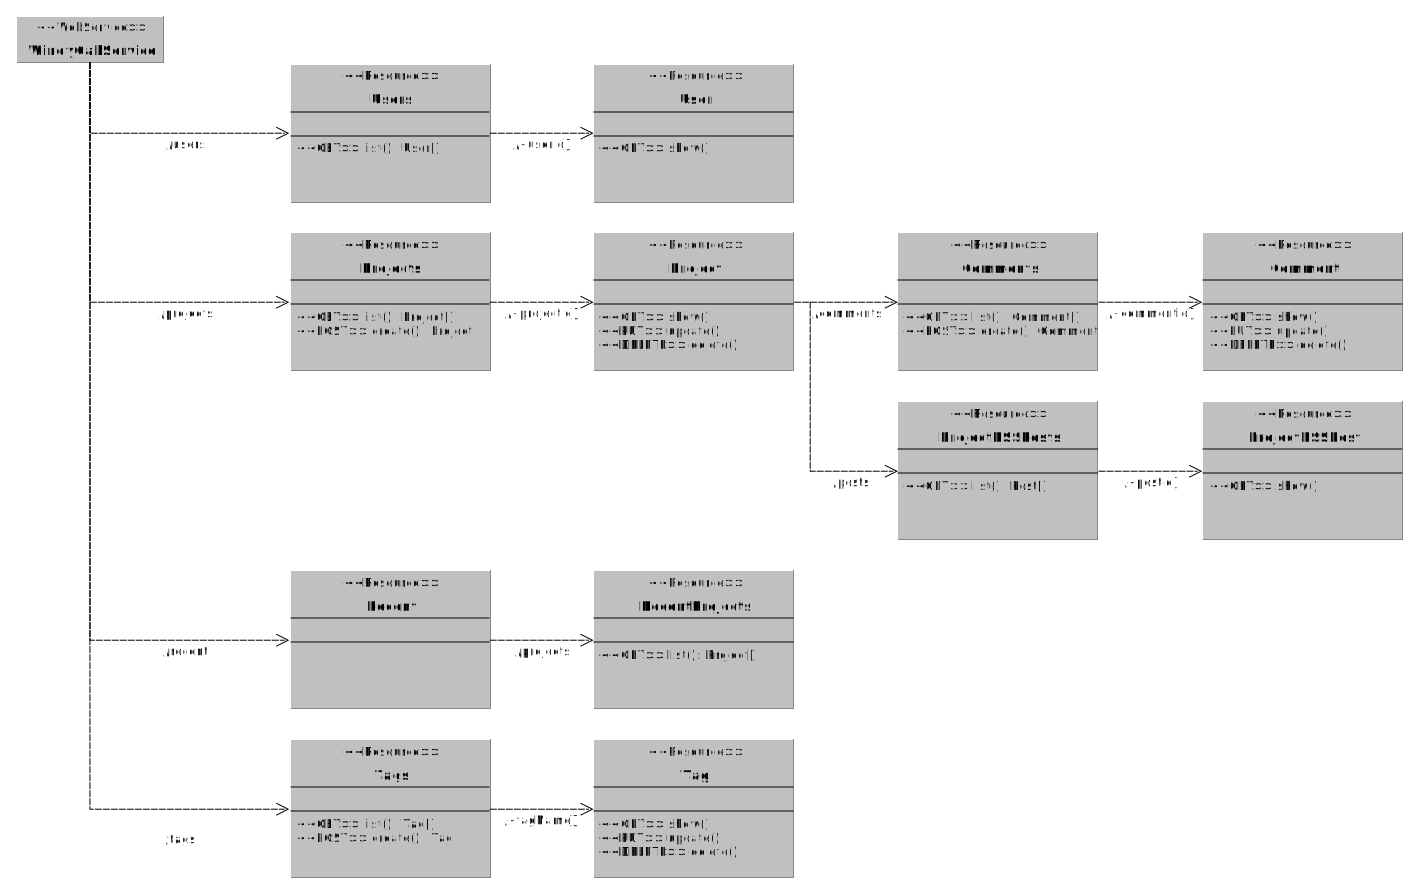
\includegraphics[height=156]{Bilder/rest.pdf} 
				\label{fig:rest}
			\end{figure}	
		\end{frame}
	\section{Testszenario}
		\begin{frame}{Testszenario}
			\begin{itemize}
				\item Client testet Funktionalität und zeigt Rückgabe als XML an
				\item Ausgabe von Statuscodes
				\item Wizard führt den Anwender
			\end{itemize}
		
		\end{frame}
		\begin{frame}{Testszenario}
		Anwendungsszenarien:
			\begin{itemize}
				\item Projekte
				\item Kommentare
				\item Tags
				\item RSS-Posts
			\end{itemize}
				
		\end{frame}
		
	\section{Live Aufrufe von einigen REST Befehlen}
		\begin{frame}{Live REST Abfragen}
			
		\end{frame}
		
	\section{Fazit oder Zusammenfassung oder so}
		\begin{frame}{Fazit oder Zusammenfassung oder so}
			
		\end{frame}
	
	
\end{document}

